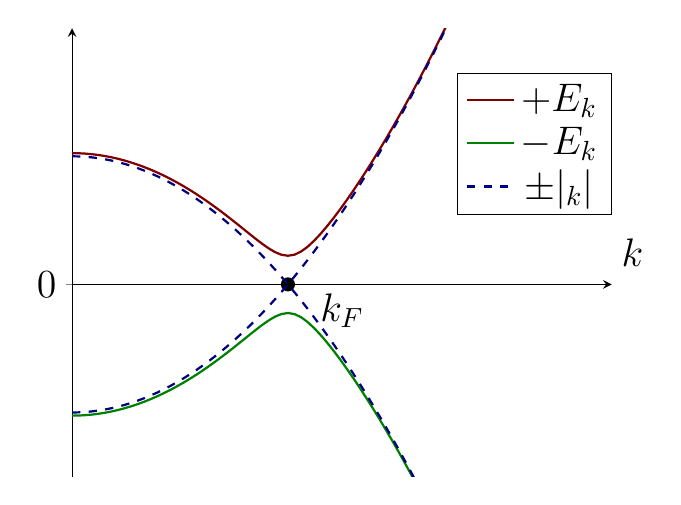
\begin{tikzpicture}

\begin{axis}[
%ticks = none,
legend style={font =\Large,at={(1,0.9)}},
ytick = {0},
yticklabels = {\Large $0$},
xtick = {0},
xticklabels ={,,},
xlabel = \Large $k$,
axis lines = left,
x label style={at={(axis description cs:1,0.5)}, anchor = west},
ymin = -1.5,
ymax= 2,
xmax = 2.5,
axis x line shift = -1.5
%y label style={at={(axis description cs:0.15,1)},rotate=-90,anchor=south},
%xlabel = $x$,
%sylabel = {$f(x)$},
]
%%Below the red parabola is defined
%\addplot [
%thick,
%domain=0:1.4, 
%samples=100, 
%color=red,
%]{1/2 * (1 + x^2 + sqrt((x^2 - 1)^2 + 0.1))};

\coordinate (b) at (axis cs:1,0) ;
\node[circle, fill, inner sep =1.8pt] at (b){};
\node[anchor = north] at (axis cs:1.25,-0.0){\Large $k_F$};


\addplot [
thick,
domain=0:3, 
samples=100, 
color=red!50!black,
]{sqrt((x^2-1)^2 + 0.05)};

\addplot [
thick,
domain=0:3, 
samples=100, 
color=green!50!black,
]{-sqrt((x^2-1)^2 + 0.05)};


\addplot [
thick,dashed,
domain=0:3, 
samples=100, 
color=blue!50!black,
]{abs((x^2-1))};
\addplot [
thick,dashed,
domain=0:3, 
samples=100, 
color=blue!50!black,
]{-abs((x^2-1))};


%%Here the blue parabloa is defined
%\addplot [
%thick,
%domain=0:1.4, 
%samples=100, 
%color=blue,
%]{1/2 * (1 + x^2 - sqrt((x^2 - 1)^2 + 0.1))};

%
%\addplot[
%thick,
%domain = 0:1.4,
%samples = 100,
%dashed
%]{1};

\addlegendentry{${+E_k}$}
\addlegendentry{$-E_k$}
\addlegendentry{$\pm |\te_k|$}
\end{axis}
\end{tikzpicture}